%   % !TEX root = ../../VIII,3_Rahmen-TeX_8-1.tex
%
%
%   Band VIII, 3 N.~??Z.1 (ex: ??A29)
%   Signatur/Tex-Datei: LH_35_10_08_015
%   RK-Nr. 60067
%   Überschrift: [De aeris resistentia elastica]
%   Modul: Mechanik / Elastizität
%   Datierung: Juli 1686
%   WZ: LEd8-Wz 803048 = RK-Wz 307 bzw. 362 (B Blume/Baum S = Gegenmarke zu Lamm in Rosette)
%   SZ: Keins
%   Bilddateien (PDF): LH_35_10_08_015_d (insgesamt: eine)
%
%
\selectlanguage{ngerman}%
\frenchspacing%
%
\begin{ledgroupsized}[r]{120mm}
\footnotesize
\pstart
\noindent\textbf{Überlieferung:}
\pend
\end{ledgroupsized}
\begin{ledgroupsized}[r]{114mm}
\footnotesize
\pstart \parindent -6mm
\makebox[6mm][l]{\textit{L}}%
Aufzeichnung: LH~XXXV~10,~8 Bl.~15.
Ein Blatt 2\textsuperscript{o};
ein Wasserzeichen: Papier möglicherweise aus dem Harz.
Eine Seite;
Bl.~15~v\textsuperscript{o} leer.
% N.~??Z.1/A29 hängt inhaltlich mit N.~??Z.2/A28 zusammen.
\pend
\end{ledgroupsized}
%
% \vspace*{5mm}
% \begin{ledgroup}
% \footnotesize
% \pstart
% \noindent\footnotesize{\textbf{Datierungsgründe:}
% Es ist nicht eindeutig, ob Leibnizens eigenhändige Datierung sich auf die Abfassung des Textes oder auf seine Randbemerkungen bezieht. ???}
% \pend
% \end{ledgroup}
%
\selectlanguage{latin}%
\frenchspacing%
%
%
\vspace{8mm}%
%
% \count\Bfootins=1200
\count\Afootins=1200
% \count\Cfootins=1200
%
\count\Bfootins=1000
\count\Cfootins=1000
%
\pstart%
\noindent%
\normalsize%
%
[15~r\textsuperscript{o}] %%%%    Blatt 15r
%
Juli 1686
\pend%
\vspace{0.5em}
%
%
%  \vspace*{1.0em}
%  \centerline{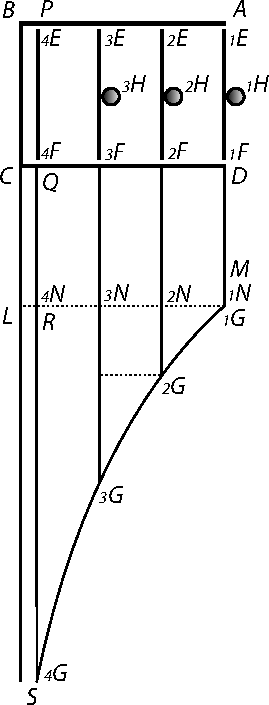
\includegraphics[width=0.30\textwidth]{gesamttex/edit_VIII,3/images/LH_35_10_08_015_d.pdf}}%\hspace*{20mm}
%  \vspace*{-1.5em}
%  \centerline{\hspace*{16mm}\lbrack\textit{Fig.~1}\rbrack}%
%  \label{LH_35_10_08_015r_Fig.1}%
%%  \vspace*{2.0em}
%  \newpage
%
%
\pstart%
\noindent%
\edtext{Embolus\protect\index{Sachverzeichnis}{embolus} \textit{EF} intruditur in vas \textit{AC},}{%
\lemma{Embolus \lbrack...\rbrack\ vas \textit{AC}}\Cfootnote{%
Siehe das Diagramm \lbrack\textit{Fig.~1}\rbrack\ auf S.~\pageref{LH_35_10_08_015r_Fig.1}.}}
%
aere\protect\index{Sachverzeichnis}{aer compressus}
%
\edtext{plenum,\protect\index{Sachverzeichnis}{vas aere plenum}
incursu corporis \textit{H}.\protect\index{Sachverzeichnis}{corpus incurrens}
Dividatur spatium \textit{CD} in partes indefinite parvas,\protect\index{Sachverzeichnis}{pars spatii infinite parva}
quales sunt \textit{{\scriptsize{1}}F{\scriptsize{2}}F}, \textit{{\scriptsize{2}}F{\scriptsize{3}}F} etc.
Et primo quidem impetu\protect\index{Sachverzeichnis}{impetus corporis incurrentis}}{%
\lemma{plenum,}\Bfootnote{%
\textit{(1)}~impetu
\textit{(2)}~incursu corporis \textit{H}
\textit{(a)}~, et primo quidem temporis articulo aliqu
\textit{(b)}~. Dividatur spatium \lbrack...\rbrack\ quidem impetu%
~\textit{L}}}
%
corpus \textit{H} incidens\protect\index{Sachverzeichnis}{corpus incidens} in \textit{{\scriptsize{1}}E{\scriptsize{1}}F}
ipsumque pellens\protect\index{Sachverzeichnis}{corpus pellens} usque ad \textit{{\scriptsize{2}}E{\scriptsize{2}}F},
perdet aliquam virium\protect\index{Sachverzeichnis}{vis pellens} suarum partem,
quam placet repraesentare per rectangulum\protect\index{Sachverzeichnis}{rectangulum} \textit{{\scriptsize{1}}G{\scriptsize{2}}F};
et secundo impetu\protect\index{Sachverzeichnis}{impetus corporis incurrentis} embolum\protect\index{Sachverzeichnis}{embolus}
pellens\protect\index{Sachverzeichnis}{corpus pellens} a \textit{{\scriptsize{2}}E{\scriptsize{2}}F} ad \textit{{\scriptsize{3}}E{\scriptsize{3}}F},
perdet aliquam partem suarum virium,\protect\index{Sachverzeichnis}{vis pellens}
quam
%
\edtext{representabimus per rectangulum\protect\index{Sachverzeichnis}{rectangulum} \textit{{\scriptsize{2}}G{\scriptsize{3}}F}.}{%
\lemma{representabimus}\Bfootnote{%
\textit{(1)}~triangulo\protect\index{Sachverzeichnis}{triangulum}
\textit{(2)}~rectan
\textit{(3)}~per rectangulum \textit{{\scriptsize{2}}G{\scriptsize{3}}F}.%
~\textit{L}}}
%
Videndum
%
\edtext{est,
quae}{%
\lemma{est,}\Bfootnote{\hspace{-0,5mm}%
\textbar~primo \textit{gestr.}~%
\textbar\ quae
~\textit{L}}}
%
sit ratio inter \textit{{\scriptsize{1}}F{\scriptsize{1}}G} et \textit{{\scriptsize{2}}F{\scriptsize{2}}G}
posito ipsas \textit{{\scriptsize{1}}F{\scriptsize{2}}F} et \textit{{\scriptsize{2}}F{\scriptsize{3}}F} esse aequales,
seu quae sit progressio ipsarum \textit{FG}.
Quod ut cognoscatur
considerandum
\edtext{est,
vim aeris\protect\index{Sachverzeichnis}{vis aeris compressi} in vaso\protect\index{Sachverzeichnis}{vas aere plenum}
qua \lbrack comprimenti\rbrack\ resistit\protect\index{Sachverzeichnis}{resistentia aeris}
aequari ponderi cylindri aerei%
\protect\index{Sachverzeichnis}{cylinder aereus}\protect\index{Sachverzeichnis}{pondus cylindri aerei}
respondentis ipsi vasi,\protect\index{Sachverzeichnis}{vas aere plenum}%
}{%
\lemma{est,}\Bfootnote{%
\textit{(1)}~primo
\textit{(a)}~impetum
\textit{(b)}~impetu aerem 
\textit{(aa)}~redi
\textit{(bb)}~in \textit{AC} comprehensum redigi in
\textit{(c)}~aerem reductum esse in spatium \textit{AC}, tanta vi, quanta est
\textit{(aa)}~cylindri ae
\textit{(bb)}~ponderis cylindro aereo aequalis
\textit{(2)}~vim aeris
\textbar~in vaso \textit{erg.}~%
\textbar\ qua
\textbar~\textlangle se\textrangle\ \textit{gestr.}~%
\textbar~comprementi \textit{ändert Hrsg.}~%
\textbar\ resistit aequari \lbrack...\rbrack\ ipsi vasi,% ponderi cylindri aerei respondentis
~\textit{L}}}
%
\edtext{ut notum est,}{%
\lemma{ut notum est}\Cfootnote{%
Gemeint sind wohl die Untersuchungen von
E.~Torricelli,\protect\index{Namensregister}{\textso{Torricelli} (Torricellius), Evangelista 1608\textendash1647}
B.~Pascal,\protect\index{Namensregister}{\textso{Pascal} (Pascalius), Blaise 1623\textendash1662}
R.~Boyle\protect\index{Namensregister}{\textso{Boyle} (Boylius, Boyl), Robert 1627\textendash1691}
und O.~von Guericke\protect\index{Namensregister}{\textso{Guericke} (Gerickius, Gerick.), Otto von 1602\textendash1686}
über den atmosphärischen Druck.
Siehe hierüber etwa \textit{LSB} VIII,~1 N.~39, S.~306.\cite{01069}
}}
%
% \edtext{\lbrack quod\rbrack}{%
% \lemma{quam}\Bfootnote{\textit{L~ändert Hrsg.}}}
%
quam repraesentemus per
%
\edtext{rectam \textit{DM}}{%
\lemma{rectam}\Bfootnote{%
\textit{(1)}~\textit{DN}
\textit{(2)}~\textit{DM}%
~\textit{L}}}
%
vel \textit{{\scriptsize{1}}F{\scriptsize{1}}G}.
Vim aeris\protect\index{Sachverzeichnis}{vis aeris compressi}
%
\edtext{vero compressi intra \textit{C{\scriptsize{2}}F} aequari alteri ponderi\protect\index{Sachverzeichnis}{pondus comprimens}}{%
\lemma{vero}\Bfootnote{%
\textit{(1)}~qua a po
\textit{(2)}~compressi intra \lbrack...\rbrack\ alteri ponderi% \textit{C{\scriptsize{2}}F} aequari
~\textit{L}}}
%
majori,
%
\edtext{cum}{%
\lemma{cum}\Bfootnote{%
\textit{erg.~L}}}
%
quo in
%
\edtext{aequilibrio\protect\index{Sachverzeichnis}{aequilibrium} teneri posset,}{%
\lemma{aequilibrio}\Bfootnote{%
\textit{(1)}~tenetur
\textit{(2)}~esse
\textit{(3)}~teneri posset,%
~\textit{L}}}
%
quod erit ad \textit{DM} in ratione \textit{CD} ad
%
\edtext{\textit{C{\scriptsize{2}}F},
et pondus
quo idem aer teneri potest compressus\protect\index{Sachverzeichnis}{aer compressus} in}{%
\lemma{\textit{C{\scriptsize{2}}F},}\Bfootnote{%
\textit{(1)}~et vim aeris compressi in
\textit{(2)}~et pondus quo
\textit{(a)}~compressus
\textit{(b)}~idem aer \lbrack...\rbrack\ compressus in% teneri potest 
~\textit{L}}}
%
\textit{C{\scriptsize{3}}F} esse ad \textit{DM}
ut \textit{CD} ad \textit{C{\scriptsize{3}}F}
et ita porro.
%
\edtext{Eaque pondera\protect\index{Sachverzeichnis}{pondus comprimens} repraesentemus per rectas \lbrack\textit{DM}\rbrack\ seu
\textit{{\scriptsize{1}}F{\scriptsize{1}}G},
\textit{{\scriptsize{2}}F{\scriptsize{2}}G},
\textit{{\scriptsize{3}}F{\scriptsize{3}}G},
ipsam \textit{LM} secantes in~\textit{N}.}{%
\lemma{Eaque}\Bfootnote{%
\hspace{-0,5mm}pondera repraesentemus per rectas
\textbar~\textit{CD} \textit{ändert Hrsg.}~%
\textbar\ seu \textit{{\scriptsize{1}}F{\scriptsize{1}}G}, \textit{{\scriptsize{2}}F{\scriptsize{2}}G}, \textit{{\scriptsize{3}}F{\scriptsize{3}}G},
\textit{(1)}~quarum differentiae sint \textit{{\scriptsize{1}}L{\scriptsize{2}}G}, \textit{{\scriptsize{2}}L{\scriptsize{3}}G} etc.
\textit{(2)}~ipsam \textit{LM} secantes in \textit{N}.
\textit{erg.~L}}}
%
\edtext{Hinc corpus}{%
\lemma{Hinc}\Bfootnote{%
\textit{(1)}~vis
\textit{(2)}~corpus%
~\textit{L}}}
%
\textit{H} ingruens\protect\index{Sachverzeichnis}{corpus ingruens}
aeremque ex \textit{CD} in \textit{C{\scriptsize{2}}F} comprimens,\protect\index{Sachverzeichnis}{corpus comprimens}
tantundem virium\protect\index{Sachverzeichnis}{vis comprimens}
%
\edtext{perdet quantum}{%
\lemma{perdet}\Bfootnote{\hspace{-0,5mm}%
\textbar~(\protect\vphantom)%
seu aeri dabit%
\protect\vphantom()
\textit{gestr.}~%
\textbar\ quantum%
~\textit{L}}}
%
perdidisset si pondus quod
%
\edtext{sit ut}{%
\lemma{sit}\Bfootnote{\hspace{-0,5mm}%
\textbar~ad pondus aeris \textit{gestr.}~%
\textbar\ ut%
~\textit{L}}}
%
\textit{{\scriptsize{2}}N{\scriptsize{2}}G}
elevasset ad altitudinem \textit{{\scriptsize{2}}F{\scriptsize{1}}F}.
Et idem corpus \textit{H} aerem\protect\index{Sachverzeichnis}{aer compressus}
%
\edtext{ex \textit{C{\scriptsize{2}}F}}{%
\lemma{ex}\Bfootnote{%
\textit{(1)}~\textit{{\scriptsize{2}}E{\scriptsize{2}}F}
\textit{(2)}~\textit{C{\scriptsize{2}}F}%
~\textit{L}}}
%
in \textit{C{\scriptsize{3}}F} comprimens,\protect\index{Sachverzeichnis}{corpus comprimens}
tantum virium perdet,\protect\index{Sachverzeichnis}{vis comprimens}
quantum perdidisset
%
\edtext{\lbrack si\rbrack}{%
\lemma{si}\Bfootnote{%
\textit{erg. Hrsg.}}}
%
pondus \textit{{\scriptsize{3}}N{\scriptsize{3}}G} elevasset ad
%
\edtext{altitudinem \textit{{\scriptsize{2}}F{\scriptsize{3}}F}.}{%
\lemma{altitudinem}\Bfootnote{%
\textit{(1)}~\textit{{\scriptsize{2}}N{\scriptsize{3}}N}
\textit{(2)}~\textit{{\scriptsize{2}}F{\scriptsize{3}}F}.%
~\textit{L}}}
%
Et ita porro.
Itaque vires\protect\index{Sachverzeichnis}{vis comprimens}
quae perduntur a corpore\protect\index{Sachverzeichnis}{corpus comprimens} \textit{H}
erunt ut ipsae \textit{NG}.
Similiter impetus\protect\index{Sachverzeichnis}{impetus aeris compressi}
%
\edtext{qui ab aere compresso,}{%
\lemma{qui}\Bfootnote{%
\textit{(1)}~a corp
\textit{(2)}~ab aere compresso,%
~\textit{L}}}
%
se restituente\protect\index{Sachverzeichnis}{aer se restituens} imprimuntur corpori \textit{H}.
\pend%
 \vspace{2.0em}
  \centerline{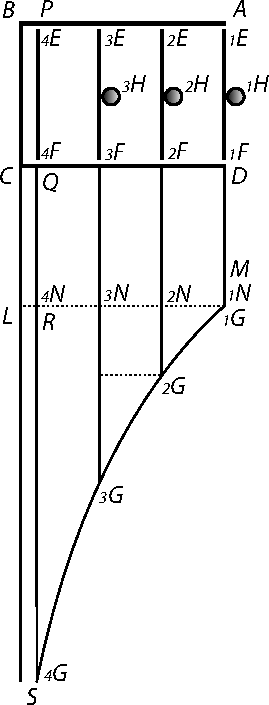
\includegraphics[width=0.29\textwidth]{gesamttex/edit_VIII,3/images/LH_35_10_08_015_d.pdf}}%\hspace*{20mm}
  \vspace{-1.0em}
  \centerline{\hspace{16mm}\lbrack\textit{Fig.~1}\rbrack}%
  \label{LH_35_10_08_015r_Fig.1}%
\newpage%
%
\pstart%
\noindent%
\lbrack\textit{Nachfolgend kleingedruckter Text in L gestrichen:}\rbrack\
\pend%
\vspace{0.5em}%
% \newpage%
\footnotesize%
\pstart%
\noindent%
%%
\edtext{Si ducatur \textit{{\scriptsize{2}}F{\scriptsize{3}}F}
in \lbrack triangulum\rbrack\ \textit{{\scriptsize{3}}G{\scriptsize{3}}N{\scriptsize{1}}N}\protect\index{Sachverzeichnis}{triangulum}
aequabitur potentiae quam corpus \textit{H} perdidit,\protect\index{Sachverzeichnis}{potentia corporis comprimentis}}{%
\lemma{Si}\Bfootnote{%
\textit{(1)}~ponamus jam in 
\textit{(a)}~\textlangle\textit{{\scriptsize{4}}}\textrangle\textit{F} seu
\textit{(b)}~\textit{Q} seu \textit{{\scriptsize{4}}F} cessare compressionem
\textit{(aa)}~ponderis
\textit{(bb)}~corporis \textit{H}, sequitur ipsius 
\textit{(aaa)}~pondus
\textit{(bbb)}~vim quam in \textlangle compri\textrangle\
\textit{(2)}~ducatur \textit{{\scriptsize{2}}F{\scriptsize{3}}F}
\textbar~in \textit{erg.}
\textbar~rectangulum \textit{ändert Hrsg.}~%
\textbar~\textit{(a)}~\textit{{\scriptsize{3}}N{\scriptsize{3}}}
\textit{(b)}~\textit{{\scriptsize{3}}G{\scriptsize{3}}N{\scriptsize{1}}N}
\textit{(aa)}~repraesentabit
\textit{(bb)}~aequabitur potentiae \lbrack...\rbrack\ \textit{H} perdidit,% quam corpus 
~\textit{L}}}
%%
datur autem \textit{{\scriptsize{3}}N{\scriptsize{3}}G},
ex datis \textit{DM} et \textit{C{\scriptsize{3}}F}
(\protect\vphantom)%
quia \textit{{\scriptsize{3}}F{\scriptsize{3}}G} est ad \textit{{\scriptsize{1}}F{\scriptsize{1}}G}
ut \textit{CD} ad \textit{C{\scriptsize{3}}F}%
\protect\vphantom()
ergo et datur vis corporis \textit{H};\protect\index{Sachverzeichnis}{vis corporis comprimentis}
quae divisa per ejus molem\protect\index{Sachverzeichnis}{moles corporis comprimentis}
%
\edtext{dabit quadratum celeritatis\protect\index{Sachverzeichnis}{quadratum celeritatis}}{%
\lemma{dabit}\Bfootnote{%
\textit{(1)}~vim
\textit{(2)}~quadratum celeritatis%
~\textit{L}}}
%
quam habuit corpus \textit{H}\protect\index{Sachverzeichnis}{corpus impingens}
cum impingeret in embolum.\protect\index{Sachverzeichnis}{embolus}
% \edlabel{LH_35_10_08_015r_petitAbszt-1}
\pend%
\pstart%
Itaque\protect\index{Sachverzeichnis}{cylinder aereus}\protect\index{Sachverzeichnis}{pondus cylindri aerei}
%
\edtext{\textit{DM} pondus cylindri aerei sit \textit{a},}{%
\lemma{\textit{DM}}\Bfootnote{%
\textit{(1)}~pondus sit \textit{a}
\textit{(2)}~pondus cylindri aerei sit \textit{a},%
~\textit{L}}}
%
altitudo \textit{CF} sit \textit{x},
erit $\displaystyle FG = aa : x$
et $\displaystyle NG = aa : x - a$
seu
\edtext{$\displaystyle\frac{aa - ax}{x},$
quae ducta in \textit{DF}, seu in $\displaystyle a - x$ dabit $\displaystyle\overline{a - x}^2 a : x,$
repraesentans vim\protect\index{Sachverzeichnis}{vis corporis comprimentis}
quae divisa per corpus \textit{H},\protect\index{Sachverzeichnis}{corpus comprimens}
seu per \textit{h},}{%
\lemma{$\displaystyle\frac{aa - ax}{x}$}\Bfootnote{%
\textit{(1)}~. Corpus \textit{H} sit \textit{h},
\textit{(2)}~, quae ducta \lbrack...\rbrack\ divisa per
\textit{(a)}~\textlangle\textit{h}\textrangle, corpus
\textit{(b)}~corpus \textit{H}, seu per \textit{h},%
~\textit{L}}}
%
dabit $\displaystyle\overline{a - x}^2 \cdot a : hx$
%
\edtext{potentiam a corpore \textit{h} adhuc acquirendam,%
\protect\index{Sachverzeichnis}{potentia acquirenda}}{%
\lemma{potentiam}\Bfootnote{%
\textit{(1)}~quam corpus \textit{h} dabit
\textit{(2)}~a corpore \textit{h} adhuc acquirendam,%
~\textit{L}}}
%
sit autem c \normalsize{\lbrack\textit{Text bricht ab.}}\rbrack\
\pend%
\pstart%
Itaque \textit{DM} pondus cylindri aerei%
\protect\index{Sachverzeichnis}{cylinder aereus}\protect\index{Sachverzeichnis}{pondus cylindri aerei}
%
\edtext{sit \textit{a}, \textit{DQ} sit \textit{q},}{%
\lemma{sit}\Bfootnote{%
\hspace{-0,5mm}\textit{a},
\textbar~et \textit{gestr.}~%
\textbar\ \textit{DQ} sit \textit{q},%
~\textit{L}}}
%
fiet \textit{QS}
(\protect\vphantom)%
seu \textit{{\scriptsize{4}}F{\scriptsize{4}}G}%
\protect\vphantom()
$\displaystyle = aa : q$
et \textit{RS} seu \textit{{\scriptsize{4}}N{\scriptsize{4}}G}
erit aeq.
%
\edtext{$\displaystyle aa : \overline{a - q} - a,$
seu $\displaystyle\protect\ovalbox{$\displaystyle aa -aa$} + aq : \overline{a - q}$
quae ducta in \textit{QF} seu in \textit{q} dabit $\displaystyle aqq : \overline{a - q}$
potentiam totam compressione quaesitam,%
\protect\index{Sachverzeichnis}{potentia compressione quaesita}\protect\index{Sachverzeichnis}{potentia aeris}
quae divisa per molem corporis \textit{H},\protect\index{Sachverzeichnis}{moles corporis comprimentis}
seu \textit{h} dabit $\displaystyle aqq : h\,\overline{a - q}.$}{%
\lemma{$\displaystyle aa : \overline{a - q} - a,$}\Bfootnote{%
\textit{(1)}~\textlangle et\textrangle\
\textit{(2)}~quae ducta in \textit{QF} seu in \textit{a}, dabit $\displaystyle aa - aq$
\textit{(3)}~seu $\displaystyle\protect\ovalbox{$\displaystyle aa -aa$} + aq : \overline{a - q}$ \lbrack...\rbrack\ dabit $\displaystyle aqq : \overline{a - q}$
\textit{(a)}~et divisa per \textit{H} seu \textit{h} molem corporis dabit
\textit{(b)}~potentiam totam compressione quaesitam, quae
\textit{(aa)}~ducta
\textit{(bb)}~divisa per molem corporis \textit{H}
\textit{(aaa)}~dabit
\textit{(bbb)}~, seu \textit{h} dabit $\displaystyle aqq : h \overline{a - q}.$%
~\textit{L}}}
%%
Si
%
\edtext{jam aliquod punctum \textit{F} sumatur}{%
\lemma{jam}\Bfootnote{%
\textit{(1)}~sit aliqua
\textit{(2)}~aliquod punctum \textit{F} 
\textit{(a)}~sit
\textit{(b)}~sumatur%
~\textit{L}}}
%
inter \textit{Q} et \textit{D},
et \textit{DF} dicatur \textit{x},
%
\edtext{erit \textit{CF}}{%
\lemma{erit}\Bfootnote{%
\textit{(1)}~\textit{DF}
\textit{(2)}~\textit{CF}%
~\textit{L}}}
%
$\displaystyle = a - x$ et $\displaystyle FG = aa : \overline{a - x}$
et $\displaystyle NG = aa : \overline{a - x} - a$ seu $\displaystyle ax : \overline{a - x}$
et $\displaystyle NGD = axx : \overline{a - x}$
potentia adhuc acquirenda.\protect\index{Sachverzeichnis}{potentia acquirenda}
\pend%
\normalsize%
\vspace{0.5em}%
%
%
%  \newpage%
%  \vspace*{0.0em}
%  \centerline{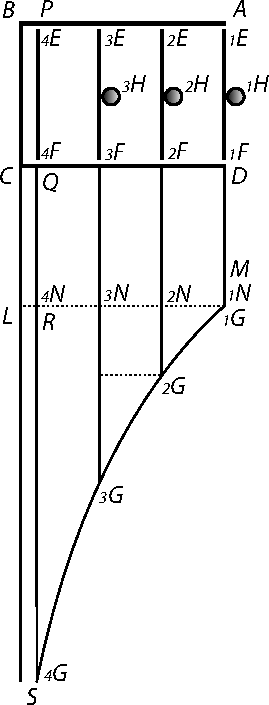
\includegraphics[width=0.28\textwidth]{gesamttex/edit_VIII,3/images/LH_35_10_08_015_d.pdf}}%\hspace*{20mm}
%  \vspace*{-1.5em}
%  \centerline{\hspace*{16mm}\lbrack\textit{Fig.~1}\rbrack}%
%  \label{LH_35_10_08_015r_Fig.1}%
%  \vspace*{2.0em}
%  \newpage
%
%
\pstart%
\noindent%
Si ponamus jam in \textit{Q}
seu in \textit{{\scriptsize{4}}F} cessare compressionem,\protect\index{Sachverzeichnis}{compressio aeris}
necesse
%
\edtext{est vim\protect\index{Sachverzeichnis}{vis aeris}
quam Elasticus aer\protect\index{Sachverzeichnis}{aer elasticus} acquisivit
seu corpus impingens\protect\index{Sachverzeichnis}{corpus impingens} perdidit
repraesentari Hyperbolico trilineo\protect\index{Sachverzeichnis}{trilineum hyperbolicum} \textit{MRSGM}
seu \lbrack\textit{M{\scriptsize{4}}NS{\scriptsize{4}}GM}\rbrack,
quod}{%
\lemma{est}\Bfootnote{%
\textit{(1)}~vim totam \textit{MD}
\textit{(2)}~vim quam Elasticus aer acquisivit
\textbar~seu corpus impingens perdidit \textit{erg.}~%
\textbar\ repraesentari
\textit{(a)}~toto spatio
\textit{(b)}~Hyperbolico trilineo \textit{MRSGM}
\textbar~seu
\textbar~\textit{M{\scriptsize{4}}N{\scriptsize{4}}GSM} \textit{ändert Hrsg.}~%
\textbar\ \textit{erg.}~%
\textbar~, quod%
~\textit{L}}}
%%%
divisum per \textit{h}
(\protect\vphantom)%
corpori \textit{H} respondentem quantitatem%
\protect\vphantom()
dabit potentiam\protect\index{Sachverzeichnis}{potentia corporis comprimentis}
%
\edtext{corporis \textit{H},
cujus quadratica radix\protect\index{Sachverzeichnis}{radix quadratica}}{%
\lemma{corporis \textit{H},}\Bfootnote{%
\textit{(1)}~quae ducta in
\textit{(2)}~cujus
\textit{(a)}~quadratum
\textit{(b)}~quadratica radix%
~\textit{L}}}
%
exprimet celeritatem\protect\index{Sachverzeichnis}{celeritas corporis comprimentis}
qua corpus \textit{H} initio ingruebat.\protect\index{Sachverzeichnis}{corpus ingruens}
Similiter, si
%
\edtext{pervenerit corpus\protect\index{Sachverzeichnis}{corpus comprimens} \textit{H} in}{%
\lemma{pervenerit}\Bfootnote{%
\textit{(1)}~\textlangle cor\textrangle\
\textit{(2)}~in
\textit{(3)}~corpus
\textit{(4)}~corpus \textit{H} in%
~\textit{L}}}
%
aliquem locum \textit{F},
sive in compressione,\protect\index{Sachverzeichnis}{compressio aeris} sive in
%
\edtext{restitutione,\protect\index{Sachverzeichnis}{restitutio aeris}
tunc spatium hyperbolicum\protect\index{Sachverzeichnis}{spatium hyperbolicum} \textit{GNRSG}}{%
\lemma{restitutione,}\Bfootnote{%
\textit{(1)}~rectilineum
\textit{(2)}~tunc
\textbar~spatium Hyperbolicum \textit{erg.}~%
\textbar\ \textit{GNRSG}%
~\textit{L}}}
%
repraesentabit potentiam quam habet corpus \textit{H};\protect\index{Sachverzeichnis}{potentia corporis comprimentis}
at trilineum Hyp. \textit{GNMG}\protect\index{Sachverzeichnis}{trilineum hyperbolicum}
repraesentabit amissam\protect\index{Sachverzeichnis}{potentia amissa} vel
(\protect\vphantom)%
in restitutione\protect\index{Sachverzeichnis}{restitutio aeris}%
\protect\vphantom()
recuperandam\protect\index{Sachverzeichnis}{potentia recuperanda} ab hoc
%
\edtext{corpore \textit{H}.\protect\index{Sachverzeichnis}{corpus comprimens}
Potentia\protect\index{Sachverzeichnis}{potentia corporis comprimentis}
quam habet}{%
\lemma{corpore \textit{H}}\Bfootnote{%
\textit{(1)}~quae
\textit{(2)}~. Potentia quam habet%
~\textit{L}}}
%
si dividatur per \textit{h},
et provenientis quaeratur radix quadratica,\protect\index{Sachverzeichnis}{radix quadratica}
habebitur
%
\edtext{celeritas praesens%
\protect\index{Sachverzeichnis}{celeritas praesens}\protect\index{Sachverzeichnis}{celeritas corporis comprimentis}}{%
\lemma{celeritas}\Bfootnote{%
\textit{(1)}~quaesita\protect\index{Sachverzeichnis}{celeritas quaesita}
\textit{(2)}~praesens%
~\textit{L}}}
%
corporis\protect\index{Sachverzeichnis}{corpus comprimens}
%
\edtext{\lbrack\textit{H}\rbrack.}{%
\lemma{\textit{h}}\Bfootnote{%
\textit{L~ändert Hrsg.}}}
%
Constat autem spatia Hyperbolica\protect\index{Sachverzeichnis}{spatium hyperbolicum}
ut \textit{DG},
esse ipsarum \textit{CF} logarithmos;\protect\index{Sachverzeichnis}{logarithmus}
ergo spatia \textit{QG} sunt logarithmi iidem 
demto logarithmo\protect\index{Sachverzeichnis}{logarithmus}
%
\edtext{ipsius \textit{CQ}, ergo}{%
\lemma{ipsius}\Bfootnote{%
\hspace{-0,5mm}\textit{CQ}, 
\textbar~seu \textit{streicht Hrsg.}~%
\textbar\ ergo%
~\textit{L}}}
%
potentia praesens\protect\index{Sachverzeichnis}{potentia praesens}
in \textit{F} est log.\,\textit{CQ}
(\protect\vphantom)%
constans%
\protect\vphantom()
demto
%
\edtext{log.\,\textit{CF}.
Porro si comparentur}{%
\lemma{log.\,\textit{CF}}\Bfootnote{%
\textit{(1)}~et spatia
\textit{(2)}~et celeritates
\textit{(3)}~. Porro si comparentur%
~\textit{L}}}
%
inter se potentiae quaesitae compressione%
\protect\index{Sachverzeichnis}{potentia compressione quaesita}
usque ad \textit{{\scriptsize{4}}F},
aut usque ad \textit{{\scriptsize{3}}F}, etc.,
eae utique sunt ut spatia usque ad \textit{D{\scriptsize{4}}G}, \textit{D{\scriptsize{3}}G},
seu ut logarithmi \textit{CF}.\protect\index{Sachverzeichnis}{logarithmus}
Ergo celeritates\protect\index{Sachverzeichnis}{celeritas corporis comprimentis}
%
\edtext{\lbrack quas\rbrack}{%
\lemma{quam}\Bfootnote{%
\textit{L~ändert Hrsg.}}}
%
corpus idem accipere potest illa vel hac restitutione,\protect\index{Sachverzeichnis}{restitutio aeris}
sunt ut horum logarithmorum quadraticae radices.\protect\index{Sachverzeichnis}{radix quadratica logarithmi}
\pend%
% \newpage%
%
\pstart%
At quid si tempora comparentur?%
\protect\index{Sachverzeichnis}{tempus compressionis}\protect\index{Sachverzeichnis}{tempus restitutionis}
Tempora sunt ut
$\displaystyle\!\!\int\!\!\llcorner1\!:\!\sqrt{\text{log.}\,CQ - \text{log.}\,CF}\lrcorner.$
Sit $\displaystyle CF = x,$
$\displaystyle CD = a,$
$\displaystyle DF = a - x.$
$\displaystyle\text{Log.}\,x = \!\!\int\!\!\!\frac{aa}{a-x}dx$
et potentia praesens%
\protect\index{Sachverzeichnis}{potentia praesens}\protect\index{Sachverzeichnis}{potentia corporis comprimentis}
in \textit{F} erit $\displaystyle\text{log.}\,X - \!\!\int\!\!\!\frac{aa}{a-x}dx$
\edtext{seu $\displaystyle\text{log.}\,X - \text{log.}\,x$}{%
\lemma{seu}\Bfootnote{\hspace{-0,5mm}%
$\displaystyle\text{log.}\,X - \text{log.}\,x$
\textit{erg.~L}}}
et celeritas\protect\index{Sachverzeichnis}{celeritas praesens}\protect\index{Sachverzeichnis}{celeritas corporis comprimentis}
%
\edtext{praesens erit ut
$\displaystyle\surd\llcorner\text{log.}\,X - \text{log.}\,x\lrcorner$}{%
\lemma{praesens}\Bfootnote{%
\hspace{-0,5mm}erit
\textbar~: \textit{streicht Hrsg.}~\textbar~%
\textit{(1)}~ut $\displaystyle\!\!\int\!\!\llcorner\text{log.}\,X - \!\!\int\!\!\!\frac{aa}{a-x}dx\lrcorner$
\textit{(2)}~ut $\displaystyle\surd\llcorner\text{log.}\,X - \text{log.}\,x\lrcorner$%
~\textit{L}}}
et tempus\protect\index{Sachverzeichnis}{tempus compressionis}\protect\index{Sachverzeichnis}{tempus restitutionis}
(\protect\vphantom)%
ei reciprocum%
\protect\vphantom()
erit
$\displaystyle 1\!:\!\sqrt{\llcorner\text{log.}\,X - \text{log.}\,x\lrcorner}$
et totum tempus\protect\index{Sachverzeichnis}{tempus imsumtum}
%
\edtext{insumptum erit ut
$\displaystyle\!\!\int\!\!\llcorner dx\!:\!\sqrt{\text{log.}\,CQ - \text{log.}\,x}\lrcorner$}{%
\lemma{insumputm}\Bfootnote{%
\hspace{-0,5mm}erit
\textbar~ut solidum\protect\index{Sachverzeichnis}{solidum} ex his compositum seu ut summa summarum\protect\index{Sachverzeichnis}{summa summarum} ex illis, seu ut
\textit{(1)}~momentum\protect\index{Sachverzeichnis}{momentum temporis}
\textit{(2)}~momenta temporum ex \textit{DM} seu \textit{gestr.}~%
\textbar\ ut $\displaystyle\!\!\int\!\!\llcorner dx : \sqrt{\text{log.}\,CQ - \text{log.}\,x}\lrcorner$%
~\textit{L}}}
%
seu ut
$\displaystyle\!\!\int\!\!\llcorner dx\!:\!\sqrt{\text{log.}\,CQ - \!\!\int\!\!\!\frac{aa}{a-x}dx}\lrcorner.$
Quod an semper sit aequale
%
\edtext{licet alia atque alia sumatur \textit{CQ}}{%
\lemma{licet}\Bfootnote{%
\hspace{-0,5mm}alia \lbrack...\rbrack\ sumatur \textit{CQ} % atque alia 
\textit{erg.~L}}}
%
dispiciendum est.\rule[-1,5mm]{0pt}{5,5mm}
Vera est Methodus,\protect\index{Sachverzeichnis}{methodus vera}
sed eam nunc absolvere non vacat.
Nec vero scio
an semper in tali hypothesi\protect\index{Sachverzeichnis}{hypothesis}
restitutio\protect\index{Sachverzeichnis}{restitutio aeris}\protect\index{Sachverzeichnis}{restitutio isochrona}
eodem tempore\protect\index{Sachverzeichnis}{tempus restitutionis} fieri debeat,
ut in illa Hypothesi\protect\index{Sachverzeichnis}{hypothesis} in
%
\edtext{qua linea \textit{GG}}{%
\lemma{qua}\Bfootnote{%
\textit{(1)}~tempora
\textit{(2)}~linea \textit{GG}%
~\textit{L}}}
%
est recta,
\edtext{quod contingit in alicujus corporis Elastici\protect\index{Sachverzeichnis}{corpus elasticum}
tensione communi,\protect\index{Sachverzeichnis}{tensio communis}
ut alibi ostensum est.}{%
\lemma{quod \lbrack...\rbrack\ est}\Cfootnote{%
Vermutlich Anspielung auf N.~8\textsubscript{5} (S.~\refpassage{LH_35_09_15_015v_isochron-1}{LH_35_09_15_015v_isochron-2}).
In diesem Entwurf hatte Leibniz im Dezember 1680 den Isochronismus der \textit{restitutio omnimoda} einer gespannten Saite nachzuweisen versucht.
% ??? A34 (De motu elaterii se restituentis) würde auch gut passen, kann aber nicht sein, weil Datierung August 1689 ist.
}}
%
Quod
%
\edtext{peculiari scheda\protect\index{Sachverzeichnis}{scheda}}{%
\lemma{peculiari scheda}\Cfootnote{%
Vermutlich N.~\ref{41153}, %??A11, 
\textit{Motuum restitutionis regula} (Dezember 1680).
Der Isochronismus der Schwingungen einer gespannten Saite wird dort (S.~\refpassage{LH_35_09_15_003r_aequdiut-1}{LH_35_09_15_003v_aequdiut-2}) mathematisch bewiesen.
Diesem Phänomen widmete sich Leibniz auch in späteren Entwürfen
wie N.~\ref{RK60301} %??A45 
und N.~\ref{RK60353} %??A46
(1690 bis 1695).}}
%
sum persecutus.
%
\pend%
 \count\Bfootins=1200
\count\Afootins=1200
\count\Cfootins=1200
%%
%%
%%  \newpage%
%  \vspace*{2.5em}
%  \centerline{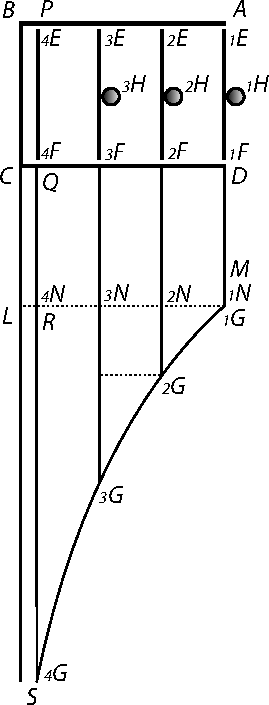
\includegraphics[width=0.28\textwidth]{gesamttex/edit_VIII,3/images/LH_35_10_08_015_d.pdf}}%\hspace*{20mm}
%  \vspace*{-1.5em}
%  \centerline{\hspace{16mm}\lbrack\textit{Fig.~1}\rbrack}%
%  \label{LH_35_10_08_015r_Fig.1}%
%%  \vspace*{2.0em}
%%  \newpage
%%
%

%
%
%%%%    Ende des <stücks auf Blatt 15r